La but du machine learning est d'acquérir un modèle à partir de données ou d'expériences. Par exemple, en apprennat des 
paramètres (probabilités), en apprenant des structures (réseaux bayésiens)...

\subsection{Classification}
\label{sub:classification}
Étant donné un point d'entrée $x$ de données avec certains features, on veut prédire une sortie $y$ qui est une classe. Voici
comment résumer cela en une ligne :
\begin{equation*}
    x(\text{input}) \rightarrow \text{features(attributs de }x) \rightarrow y(\text{output})
\end{equation*}
Le machine learning intervient entre l'étape de features et l'étape de prédiction. L'idée d'un algorithme de machine learning
est d'apprendre les pattern entre les features et les classes depuis des données. Les données (d'entraînement) sont des exemples
qui ont été préalablement classifiés.
\begin{example}
    Spam Filter :
    \begin{itemize}[label=\textbullet]
        \item input : un mail
        \item output : spam ou non spam
    \end{itemize}
    Le but est d'avoir en amont un grand nombre de mails labélisés en tant que spam ou non spam (cette action doit être faite par
    quelqu'un). Ensuite, on rajoute des features :
    \begin{itemize}[label=\textbullet]
        \item On peut rajouter des mots clés (free, money, ...)
        \item Des patterns de texte (trop de majuscules, trop de points d'exclamation, ...)
        \item ...
    \end{itemize}
\end{example}

\subsection{Model-based classification}
\label{sub:model_based_classification}
Un peu comme dans la section précédente, il y a une distinction entre les $model-free$ et les $model-based$. Donc ici, le but
est de construire un modèle ou les classes d'output et les features d'input sont des variables aléatoires. Il y aura des 
connexions entre les variables. 

\subsubsection{Naïve Bayes Model}
\begin{figure}[H]
    \centering
    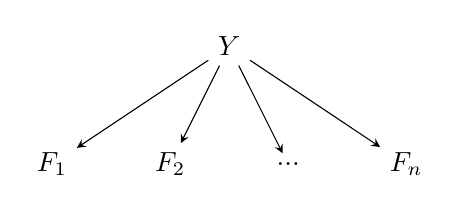
\begin{tikzpicture}[-stealth, node distance=1.5cm]
        \node {$Y$}
            child {node {$F_1$}}
            child {node {$F_2$}}
            child {node {$...$}}
            child {node {$F_n$}
            };
    \end{tikzpicture}
    \caption{Réseau de Bayes naïf}
\end{figure}
$Y$ est la classe, $F_1, F_2, ..., F_n$ sont les features. Les tables de probabilités sont les suivantes :
\begin{itemize}[label=\textbullet]
    \item $P(Y)$ : probabilité que chaque classe apparaisse sans savoir les features.
    \item $P(F_i|Y)$ : Une table par feature, probabilité de distribution d'un feature étant donné une classe.
\end{itemize}
\begin{enumerate}
    \item Pour \textbf{l'entrainement} :\\
    On utilise un jeu de données pour apprendre les tables de probabilités, pour estimer $P(Y)$, on regarde le nombre de fois
    qu'il apparaît dans le jeu de données. Pour estimer $P(F_i|Y)$, on regarde comment la classe affecte le feature.
    \item Pour \textbf{la classification} :\\
    On instantie toutes les features, on connait les input features. Pour $P(Y|F_1, F_2, ..., F_n)$, on utilise un algorithme
    d'inférence pour caculer.
\end{enumerate}
Pour un réseau de Bayes naïf, on a :
\begin{equation*}
    P(Y,F_1,\dots,F_n) = P(Y) \prod_{i=1} P(F_i|Y)
\end{equation*}
\begin{itemize}
    \item $P(Y)$ : contient $|Y|$ paramètres.
    \item $P(Y,F_1,\dots,F_n)$ : contient $|Y| \times |F|^n$ paramètres.
    \item $P(F_i|Y)$ : contient $n\times |Y| \times |F|$ paramètres.
\end{itemize}

\begin{example}
    Réseau de Bayes naïf pour la reconnaissance de chiffre :\\

    On suppose que toutes les features sont indépendantes de la classe. Ce n'est pas logique mais cela fonctionne très bien.
    Dans le cas de la reconnaissance des chiffres, il y a un feature $F_{ij}$ pour chaque position dans la grille $i,j$. Par
    exemple pour 1, on a :
    \begin{equation*}
        1 \rightarrow \langle F_{0,0}=0, F_{0,1}=0,F_{0,2}=1,F_{0,3}=1,F_{0,4}=0\dots F_{15,15}=0\rangle
    \end{equation*}
    Le modèle de Bayes naïf sera donc :
    \begin{equation*}
        P(Y|F_{0,0}, F_{0,1}, ..., F_{15,15}) \propto P(Y) \prod_{i,j} P(F_{i,j}|Y)
    \end{equation*}
    \begin{figure}[H]
        \centering
        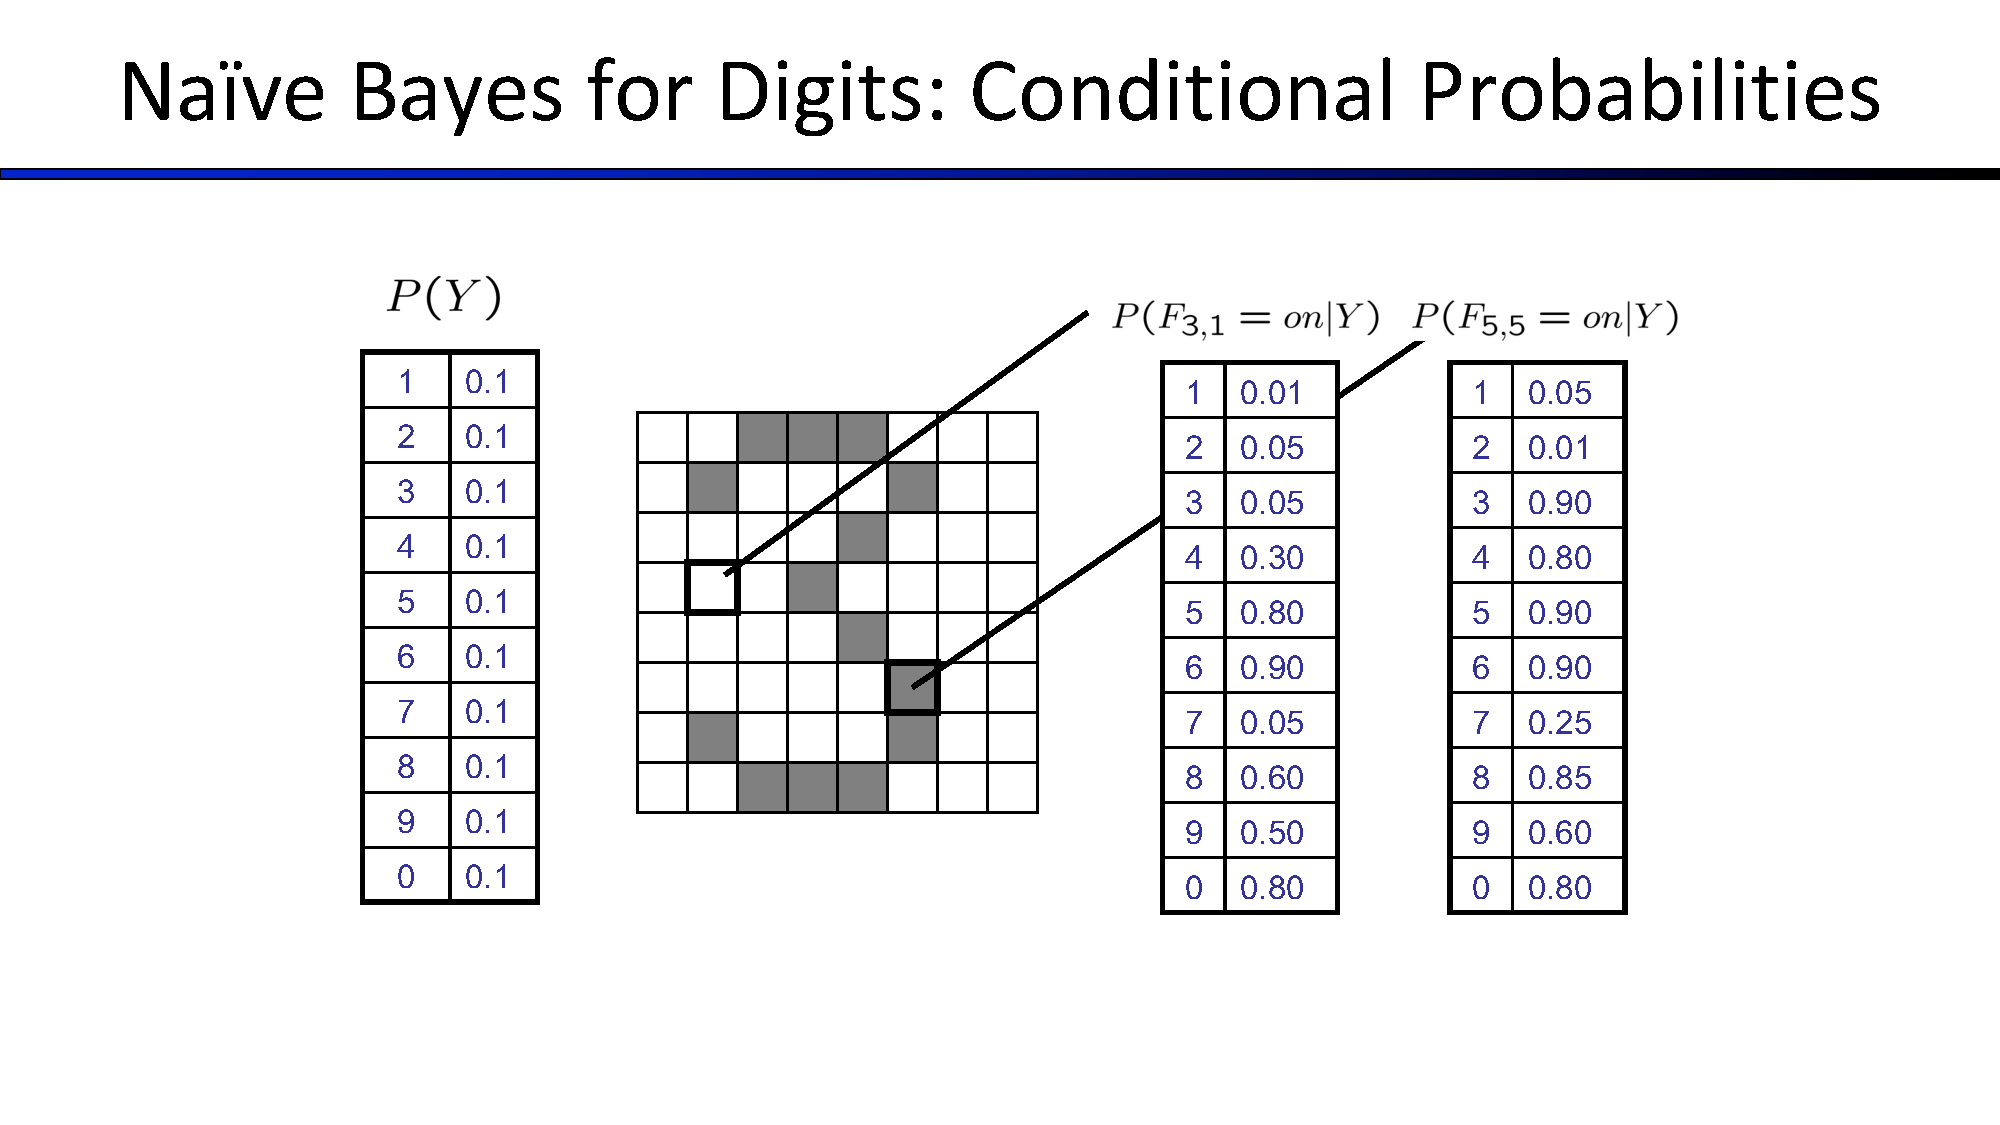
\includegraphics[width=\linewidth]{pictures/digit_recognition.pdf}
        \caption{Probabilités conditionnelles pour la reconnaissance de chiffre}
    \end{figure}
\end{example}

\subsubsection{Inference for Naïve Bayes}
Le but est de calculer $P(Y|F_1, F_2, ..., F_n)$ mais on sait qu'on peut utiliser la probabilité jointe :
\begin{equation}
    P(Y,f_1\dots f_n) =
    \begin{bmatrix}
        P(y_1,f_1...f_n)\\
        P(y_2,f_1...f_n)\\
        \vdots\\
        P(y_n,f_1...f_n)
    \end{bmatrix}
    \Rightarrow
    \begin{bmatrix}
        P(y_1)\prod_{i} P(f_i|y_1)\\
        P(y_2)\prod_{i} P(f_i|y_2)\\
        \vdots\\
        P(y_n)\prod_{i} P(f_i|y_n)
    \end{bmatrix}   
\label{eq:jointProb}
\end{equation}
Ensuite, on somme tout pour avoir la probabilité de l'évidence :
\begin{equation}
    P(f_1\dots f_n) = \sum_{i} P(y_i)\prod_{i} P(f_i|y_i)
\label{eq:evidence}
\end{equation}
Finalement, on normalise en divisant (\ref{eq:jointProb}) par (\ref{eq:evidence}) et on retrouve $P(Y|f_1\dots f_n)$.